%% A notation of one's own
%
% Styles named for what they mean, built on the package's, in the preamble or
% a notation file; a figure then uses them as it uses the package's own,
% as a type in \tnlayer and an edge type in edge=. Here a state in Vidal's
% form: tensors and the weights on the bonds between them.
\documentclass[border=4pt]{standalone}
\usepackage{tikz-tensors}
\tikzset{
  site/.style   = {tn circle, tn fill=blue1},
  weight/.style = {tn diamond, tn small, tn fill=green1},
  phys/.style   = {tn wavy, draw=warm2},
}
\begin{document}
\begin{tikzpicture}
  \tnstack{S}{5}{a}
  \tnlayer{S}{a}{site/$\Gamma$, weight/$\lambda$, site/$\Gamma$, weight/$\lambda$, site/$\Gamma$}
  \tnconnect{S}
  \tnopen[edge=phys]{down}{S-a-1, S-a-3, S-a-5}
\end{tikzpicture}
\end{document}
